\documentclass[12pt]{article}
\usepackage[utf8]{inputenc}
\usepackage{amsmath}
\usepackage{geometry}
\usepackage{hyperref}
\usepackage{xcolor} 
\usepackage{graphicx}

\geometry{a4paper, margin=1in}

\title{Autonome Stromversorgung des Jetson Orin Nano für Objekterkennung}
\author{}
\date{}

\begin{document}

\maketitle

\section{Einleitung}
Um den NVIDIA Jetson Orin Nano autonom zu betreiben, ist eine geeignete Stromquelle erforderlich, 
die das Developer-Kit ausschließlich über den Barrel-Jack mit 19 V versorgt, 
die sowohl die Anforderungen des Jetson-Boards als auch den Energieverbrauch 
während der dauerhaften Objekterkennung deckt. In dieser Arbeit werden die Energieanforderungen 
des Jetson Orin Nano untersucht. Das mitgelieferte Netzteil liefert 19.0 V und 2.37 A als Ausgang, 
was für die Versorgung des Kits ideal ist. Laut \textcolor{blue}{\href{https://developer.download.nvidia.com/assets/embedded/secure/jetson/orin_nano/docs/Jetson-Orin-Nano-DevKit-Carrier-Board-Specification_SP-11324-001_v1.2.pdf?KmgI9RJCufnwzXmxbGPExVQp1r131wrAPSzR9RMDhh83EhjqXKmYVbjwEjUNXPMiO3peL2R_7D_xp9mFQTBkPF-Bon3l72rEZPIiNTVUv5oIjQsvFsQ0pqAZxr16W-12GNU3N596RY1rC1tgxd5_XwyvJRNhcRcOank-v-QwQweH0clhI5Vvdy5dZVF-qYLeuslCScepJxD-v-TAHS2XuNFpJb69-WoTOPi_AyxiG2scwgKnqQ==&t=eyJscyI6IndlYnNpdGUiLCJsc2QiOiJkZXZlbG9wZXIubnZpZGlhLmNvbS9lbWJlZGRlZC9kb3dubG9hZHMjP3NlYXJjaD1EYXRhJTIwU2hlZXRcdTAwMjZ0eD0kcHJvZHVjdCxqZXRzb25fYWd4X29yaW4samV0c29uX29yaW5fbngsamV0c29uX29yaW5fbmFubyJ9}{NVIDIA}} 
unterstützt das Kit einen Versorgungsspannungsbereich von 9 V bis 20 V und hat einen Leistungsbedarf 
zwischen 7 W und 15 W, mögliche Batterien und Powerbanks zur Stromversorgung vorgestellt und berechnet, 
wie lange der Jetson Orin Nano bei kontinuierlicher Objekterkennung betrieben werden kann.

\section{Strombedarf des Jetson Orin Nano}
Der Strombedarf des Jetson Orin Nano hängt von der Auslastung des Systems ab. 
Im Allgemeinen wird er in folgenden Bereichen liegen:

\begin{itemize}
    \item \textbf{Leerlauf}: 5-7 W
    \item \textbf{Moderate Last}: 7-10 W
    \item \textbf{Maximale Leistung}: 15 W 
\end{itemize}

Für Anwendungen wie die Objekterkennung (z.B. YOLO, SSD) wird der Verbrauch 
\indent typischerweise im Bereich von 10 bis 15 W liegen.

\subsection{Stromversorgung}
Der Jetson Orin Nano 8GB und das Jetson Orin Nano Developer Kit unterscheiden 
sich in ihren Anforderungen an die Stromversorgung, wobei der Jetson Orin Nano 
8GB seine Stromversorgung direkt über das Developer Kit bezieht:
\begin{itemize}
    \item \textbf{Jetson Orin Nano 8GB}: Dieses Modell benötigt eine stabile 
    Eingangsspannung von \textbf{5V}. Es wird über das Developer Kit mit Strom versorgt.
    \item \textbf{Jetson Orin Nano Developer Kit}: Das Developer Kit selbst kann 
    ausschließlich über den Barrel-Jack betrieben werden und unterstützt einen 
    Eingangsspannungsbereich von \textbf{9V bis 20V}. Der Strombedarf des Kits liegt je 
    nach Leistungskonfiguration zwischen \textbf{7W und 15W}.
\end{itemize}
Dieser Unterschied ist entscheidend bei der Wahl der Stromquelle, da das Developer 
Kit die Spannungsversorgung des Jetson Orin Nano 8GB sicherstellt und zusätzlich den 
breiteren Spannungsbereich unterstützt.

\section{Energiequelle: Batterie oder Powerbank}

\subsection{Powerbank}
Eine Powerbank ist eine einfache Lösung, um den Jetson Orin Nano autonom zu betreiben. 
Die Powerbank sollte folgende Eigenschaften aufweisen:
\begin{itemize}
    \item \textbf{Unterstützung von USB-PD (Power Delivery)}: Sie sollte 15W bei 9V 
    
    liefern können.
    \item \textbf{Kapazität}: Um den Jetson für längere Zeit autonom zu betreiben, 
    sollte die Powerbank eine hohe Kapazität besitzen.
\end{itemize}

\subsection{Beispielrechnung für Powerbank}
Wenn die Powerbank eine Kapazität von 12V und 5200 mAh (entspricht 62.4 Wh) hat und der 
Jetson Orin Nano 15 W verbraucht, lässt sich die Betriebsdauer wie folgt berechnen:

\[
\text{Betriebsdauer} = \frac{\text{Kapazität der Powerbank in Wh}}{\text{Leistungsbedarf des Jetson Orin Nano in W}}
\]

Für diese Powerbank ergibt sich:
\[
\text{Betriebsdauer} = \frac{62.4 \, \text{Wh}}{15 \, \text{W}} \approx 4.16 \, \text{Stunden}
\]

Dies zeigt, dass die Powerbank den Jetson Orin Nano bei einer Leistung von 15 W 
\indent für ungefähr 4 Stunden und 10 Minuten betreiben kann. Beachten Sie, dass Effizienz- 
\indent verluste des Spannungswandlers und andere Verbraucher im System diese Laufzeit 
\indent verringern können.

\subsection{Batterie}
Eine Li-Ion oder LiFePO4-Batterie bietet eine weitere Möglichkeit, den Jetson Orin Nano 
autonom zu betreiben. Typische Parameter einer solchen Batterie:
\[
\begin{aligned}
    &\textbf{Spannung:} \quad 12V \text{ bis } 19V \\
    &\textbf{Kapazität:} \quad 12V \cdot 20Ah \approx 240Wh.
\end{aligned}
\]


\subsubsection{Beispielrechnung für Batterie}
Wenn die Batterie eine Kapazität von 240 Wh hat und der Jetson Orin Nano 15 W verbraucht, 
lässt sich die Betriebsdauer wie folgt berechnen:
\[
\text{Betriebsdauer} = \frac{240}{15} \approx 16 \, \text{Stunden}
\]

% \section{Optimierung der Energieeffizienz}

% \subsection{Energiemodi des Jetson Orin Nano}
% Der Jetson Orin Nano bietet verschiedene Energiemodi, um den Energieverbrauch zu steuern:
% \begin{itemize}
%     \item \textbf{Standardleistung}: 
%     \begin{verbatim}
%     sudo nvpmodel -m 0
%     \end{verbatim}
%     Maximale Leistung (ca. 15 W).
    
%     \item \textbf{Energiesparmodus}: 
%     \begin{verbatim}
%     sudo nvpmodel -m 1
%     \end{verbatim}
%     Reduziert den Verbrauch auf etwa 7-10 W.
    
%     \item \textbf{Taktrate anpassen}: 
%     \begin{verbatim}
%     sudo jetson_clocks --show
%     sudo jetson_clocks --store
%     \end{verbatim}
%     Optimiert die Taktraten für den Energieverbrauch.
% \end{itemize}

% \subsection{Peripheriegeräte}
% Reduziere den Energieverbrauch, indem du nicht benötigte Peripheriegeräte 
% (z.B. Monitor, Tastatur, USB-Geräte) abschaltest.

\clearpage

\section{Messung des Energieverbrauchs}
Um den tatsächlichen Energieverbrauch des Jetson Orin Nano zu messen, kann man folgende 
Tools verwenden:
\begin{itemize}
    \item \textbf{Software-Tools auf dem Jetson}:
    \begin{verbatim}
    tegrastats
    \end{verbatim}
    Dieses Tool zeigt die CPU-, GPU- und RAM-Auslastung sowie den Energieverbrauch in 
    Echtzeit.

    \begin{verbatim}
        Jetson GUI
    \end{verbatim}

    \item \textbf{Externe Messgeräte}: 
    \begin{verbatim}
        Multimeter
\end{verbatim}

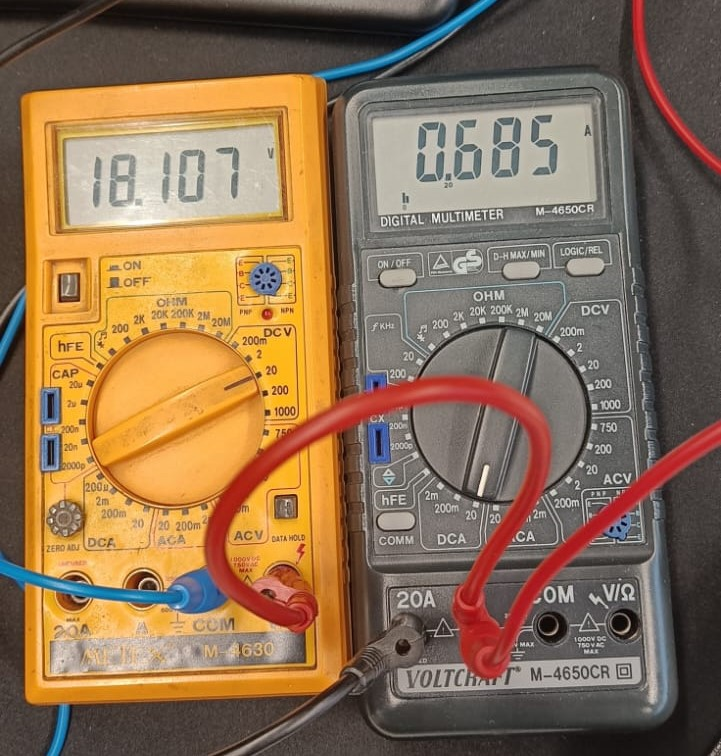
\includegraphics[width=0.8\textwidth]{Bilder/Multimeter_Messung.jpeg}

Man kann den Multimeter nutzen, um den verbrauchten Strom zu ermitteln.

\subsection*{Ergebnisse der Messung mit Multimeter}

Die Messungen des Stromverbrauchs des Jetson Orin Nano mit einem Multimeter 
ergaben folgende Werte:
\begin{itemize}
    \item \textbf{Beim Hochlaufen des Jetsons}: Der Stromverbrauch lag bei \textbf{0.9 A}.
    \item \textbf{Im Leerlauf}: Der Stromverbrauch betrug \textbf{0.4 A}.
    \item \textbf{Während der Objekterkennung}: Der Stromverbrauch stieg auf \textbf{0.8 A}.
\end{itemize}

\subsection*{Netzkabel-Test}

Der Jetson wurde mit einem Netzkabel getestet, das eine Spannung von \textbf{12V} und 
eine Stromstärke von \textbf{900mA} liefert. 
Selbst während der Objekterkennung hatte der Jetson keine Probleme mit dieser 
Stromversorgung.

    \end{itemize}
    \section{Zusammenfassung}

    Der Jetson Orin Nano benötigt eine Spannung von \textbf{12V}, wobei der 
    Stromverbrauch typischerweise bei \textbf{1A} liegt, was einer Leistung 
    von \textbf{12W} entspricht. Für einen stabilen Betrieb wird empfohlen, eine
    Energiequelle zu verwenden, die bis zu \textbf{2A} liefern kann, um Lastspitzen und 
    zusätzliche Peripheriegeräte abzudecken.
    
    Für kürzere Tests kann eine Powerbank mit \textbf{12V Ausgang} und einer 
    Kapazität von mindestens \textbf{5.200 mAh} verwendet werden. 
    
    \subsection*{Beispiel: Nutzung einer Powerbank mit 12V und 5.200mAh}
    
    Die Kapazität der Powerbank in Wattstunden (Wh) berechnet sich wie folgt:
    \[
    \text{Energieinhalt} = \text{Spannung (V)} \times \text{Kapazität (Ah)} = 12 \, \text{V} \times 5.2 \, \text{Ah} = 62.4 \, \text{Wh}
    \]
    
    Der Jetson Orin Nano benötigt im Betrieb eine Leistung von 12W. Die Laufzeit kann 
    daher berechnet werden als:
    \[
    \text{Laufzeit (h)} = \frac{\text{Energieinhalt (Wh)}}{\text{Leistungsaufnahme (W)}} = \frac{62.4}{12} \approx 5.2 \, \text{Stunden}
    \]
    
    \subsection*{Empfehlung für längeren Betrieb}
    
    Für längeren autonomen Betrieb empfiehlt sich eine Powerbank mit einer großen 
    Kapazität wie z.b. 20Ah was 20 Stunden Betribsdauer heißt.
    Eine geeignete Batterie mit großer Kapazität kann auch eine Lösung sein.

\section{Quellen}
\begin{itemize}
    \item \textcolor{blue}{\href{https://developer.download.nvidia.com/assets/embedded/secure/jetson/orin_nano/docs/Jetson-Orin-Nano-DevKit-Carrier-Board-Specification_SP-11324-001_v1.2.pdf?KmgI9RJCufnwzXmxbGPExVQp1r131wrAPSzR9RMDhh83EhjqXKmYVbjwEjUNXPMiO3peL2R_7D_xp9mFQTBkPF-Bon3l72rEZPIiNTVUv5oIjQsvFsQ0pqAZxr16W-12GNU3N596RY1rC1tgxd5_XwyvJRNhcRcOank-v-QwQweH0clhI5Vvdy5dZVF-qYLeuslCScepJxD-v-TAHS2XuNFpJb69-WoTOPi_AyxiG2scwgKnqQ==&t=eyJscyI6IndlYnNpdGUiLCJsc2QiOiJkZXZlbG9wZXIubnZpZGlhLmNvbS9lbWJlZGRlZC9kb3dubG9hZHMjP3NlYXJjaD1EYXRhJTIwU2hlZXRcdTAwMjZ0eD0kcHJvZHVjdCxqZXRzb25fYWd4X29yaW4samV0c29uX29yaW5fbngsamV0c29uX29yaW5fbmFubyJ9}{Jetson Orin Nano Developer-Kit Datasheet}}
    \item \textcolor{blue}{\href{https://developer.download.nvidia.com/assets/embedded/secure/jetson/orin_nx/docs/Jetson_Orin_NX_Series_and_Orin_Nano_Series_Design_Guide_DG-10931-001_v0.99.pdf?-ui8gdVNlYdmaR5WwGz-6xSE6JTrbPKmmiEaqjr9WzfO6o67G4dBKQu1cLXoFzsc2V3V4YrEuGoG5PmGBTp4DMwUibOm-PJI1TdO2lRc9sRcgO2NXf9KLdLphKAuH52nKmnexBGeYp2NIY0mCgF5LX7VctB_s_CeaxlaY_7BUog4ox6tD_iH2ZcG210QVnzdAVQuxdxAKdzFfO5YgnjsWnhPKu6q1_8wzr7B6rrkjGc2l6kfw5vPjg==&t=eyJscyI6IndlYnNpdGUiLCJsc2QiOiJkZXZlbG9wZXIubnZpZGlhLmNvbS9lbWJlZGRlZC9kb3dubG9hZHMjP3NlYXJjaD1EYXRhJTIwU2hlZXRcdTAwMjZ0eD0kcHJvZHVjdCxqZXRzb25fYWd4X29yaW4samV0c29uX29yaW5fbngsamV0c29uX29yaW5fbmFubyJ9}{Jetson Orin Nano Design Guide}}
\end{itemize}

\end{document}
